% vim: set tw=78 tabstop=4 shiftwidth=4 aw ai:
\documentclass{beamer}

\usepackage[utf8x]{inputenc}		% diacritice
\usepackage[english]{babel}
\usepackage{color}			% highlight
\usepackage{alltt}			% highlight
\usepackage{subfigure}
\usepackage{tikz}

% highlight; comment this out in case you don't input code source files
%\usepackage{code/highlight}		% highlight

\usepackage{hyperref}			% folositii \url{http://...}
					% sau \href{http://...}{Nume Link}
\usepackage{verbatim}

\mode<presentation>
{ \usetheme{Berlin} }

% incarcarea simbolurilor Unicode romanesti inn titlu sii primele pagini
\PreloadUnicodePage{200}

\title[SPRINT: Social Prediction-Based Opportunistic Routing]{SPRINT: Social Prediction-Based Opportunistic Routing}
\institute{Automatic Control and Computers Faculty,\\
	University Politehnica of Bucharest}
\author[R.I. Ciobanu, C. Dobre, V. Cristea]{Radu-Ioan Ciobanu, \textbf{Ciprian Dobre}, Valentin Cristea}
\date{June 4, 2013}

\begin{document}

% Slide-urile cu mai multe parti sunt marcate cu textul (cont.)
\setbeamertemplate{frametitle continuation}[from second]

% aratam numarul frame-ului
% \setbeamertemplate{footline}[frame number]

\frame{\titlepage}

\frame{\tableofcontents}

% NB: Sectiunile nu sunt marcate vizual, ci doar apar in cuprins
\section{Introduction}

% Titlul unui frame se specifica fie in acolade, imediat dupa \begin{frame},
% fie folosind \frametitle
\begin{frame}{SPRINT}
	\begin{itemize}
		\item Social PRedIction-based routing in opportunistic NeTworks
		\item introduces online social information about nodes (e.g. Facebook, Twitter, LinkedIn) as routing criterion
		\item in certain environment types, contacts between mobile devices are highly predictable
		\item prediction component approximates human mobility as a Poisson distribution when users follow rare events-based mobility patterns
		\item compare with BUBBLE Rap on real-life traces and mobility models
	\end{itemize}
\end{frame}

\section{Contact Prediction}
\begin{frame}{Contact Prediction [1]}
	\begin{itemize}
		\item try to predict a node's future behavior
		\item number of encounters and contact duration in an academic environment are regular
		\item model contacts per hour in a day as a Poisson distribution
		\item prove the assumptions using the chi-squared test
	\end{itemize}
	
	\begin{figure}[!t]
		\centering
		\subfigure[Chi-squared tests]{
			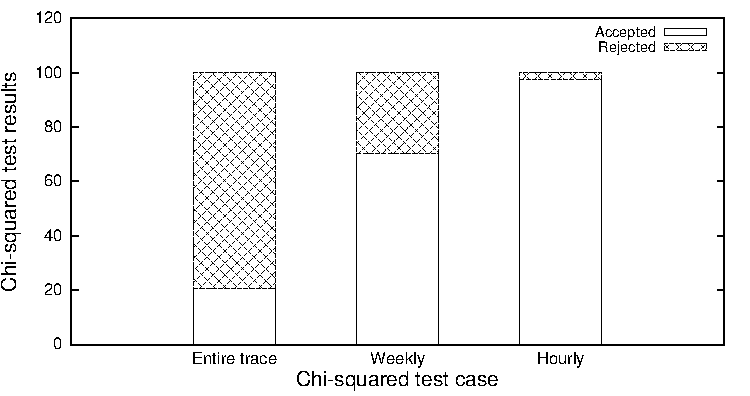
\includegraphics[width=1.7in]{img/chisquare}
			\label{fig:chisquare}
	 	}
		\subfigure[Prediction success]{
			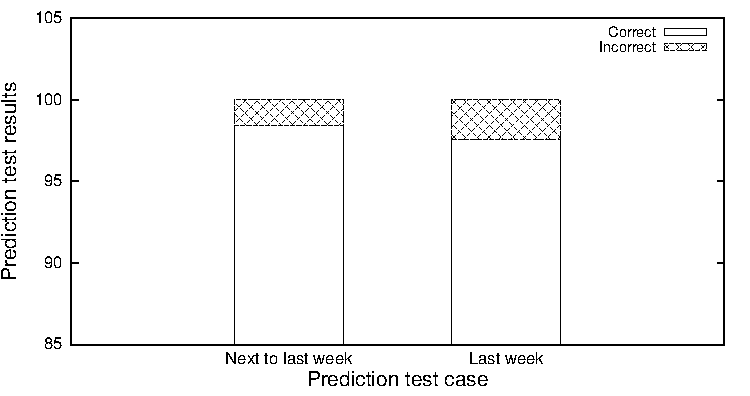
\includegraphics[width=1.7in]{img/predictions}
			\label{fig:prediction}
		}
		\label{fig:predictability}
	\end{figure}
	
	\tiny{[1] Radu Ioan Ciobanu and Ciprian Dobre. 2012. Predicting encounters in opportunistic networks. In \emph{Proceedings of the 1st ACM Workshop on High Performance Mobile Opportunistic Systems} (HP-MOSys '12).}
\end{frame}

\section{SPRINT}
\begin{frame}{The SPRINT Algorithm}
	\begin{itemize}
		\item SPRINT nodes have data memory (messages) and cache memory (contact history)
		\item on contact, they exchange information about their messages:
		\begin{itemize}
			\item hash of the content
			\item source
			\item destination
			\item generation time
			\item hop count
		\end{itemize}
		\item each node $A$ computes the utility of each message $M$ and attempts to maximize its data memory:
	\end{itemize}
	
	\hskip0.5in
	\small{
		\begin{beamerboxesrounded}[lower=block body,shadow=true,width=3.2in]{}
			\begin{center}
				\texttt{$u(M, A) = w_1 * U_1(M, A) + w_2 * U_2(M, A)$}
			\end{center}
		\end{beamerboxesrounded}
	}
\end{frame}

\begin{frame}{The SPRINT Algorithm (2)}
	\hskip0.5in
	\small{
		\begin{beamerboxesrounded}[lower=block body,shadow=true,width=3.2in]{}
			\begin{center}
				\texttt{$U_1(M, A) = freshness(M) + p(M, A) * (1 - \frac{enc(M, A)}{24})$}
			\end{center}
		\end{beamerboxesrounded}
	}
	
	\begin{itemize}
		\item $freshness(M)$ $\rightarrow$ favors newer messages (0 if message is older than one day, 0.5 otherwise)
		\item $p(M,A)$ $\rightarrow$ probability of node $A$ being able to deliver message $M$:
		\begin{itemize}
			\item count how many time each node was encountered
			\item if the node was met in the same week-day and two-hour interval, increase value by 1
			\item if the node is socially-connected, double the value
			\item compute encounter probability as ratio between contacts with each node and total contacts
			\item compute number of encounters $N$ for each of the next 24 hours using Poisson (choose first $N$, $\lambda$ $\rightarrow$ max likelihood)
		\end{itemize}
		\item $enc(M,A)$ $\rightarrow$ time (h) until $M$'s destination will be met by $A$
	\end{itemize}
\end{frame}

\begin{frame}{The SPRINT Algorithm (3)}
	\hskip0.5in
	\small{
		\begin{beamerboxesrounded}[lower=block body,shadow=true,width=3.2in]{}
			\begin{center}
				\texttt{$U_2(M, A) = c_e(M, A) * \frac{s_n(M) + hop(M) + pop(A) + t(M, A)}{4}$}
			\end{center}
		\end{beamerboxesrounded}
	}
	
	\begin{itemize}
		\item $c_e(M, A)$ $\rightarrow$ 1 if $A$ is socially-connected with $M$'s destination, or if it will encounter a node that has a social relationship with $M$ in the next 24 hours, 0 otherwise
		\item $s_n(M)$ $\rightarrow$ 1 if $M$'s source and destination are not socially-connected, 0 otherwise
		\item $hop(M)$ $\rightarrow$ normalized number of nodes visited by $M$
		\item $pop(A)$ $\rightarrow$ $A$'s social popularity (e.g. number of Facebook friends)
		\item $t(M, A)$ $\rightarrow$ normalized time spent by $A$ in contact with $M$'s destination
	\end{itemize}
\end{frame}

\begin{frame}{The SPRINT Algorithm (3)}
	\begin{figure}[!t]
		\centering
		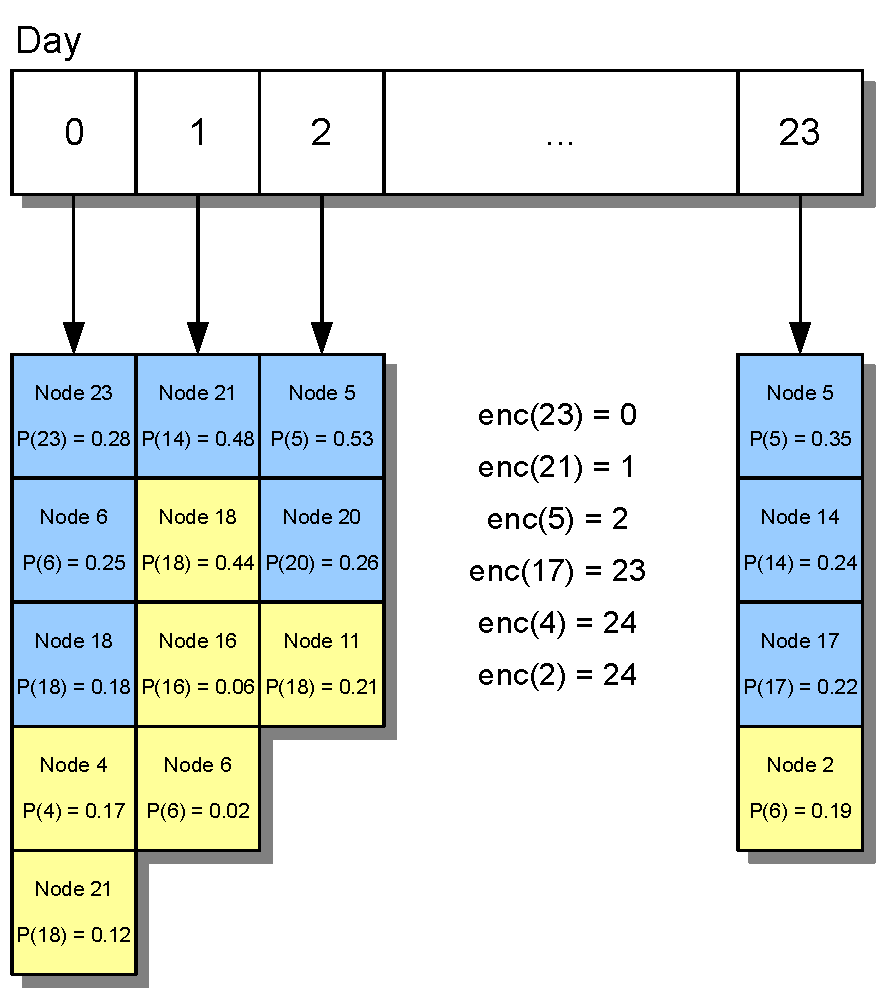
\includegraphics[scale=0.4]{img/prediction}
	\end{figure}
\end{frame}

\section{Experimental Results}

\begin{frame}{Mobility Traces and Models}
	\begin{itemize}
		\item UPB 2011:
		\begin{itemize}
			\item faculty grounds
			\item Bluetooth
			\item 35 days, 22 participants
		\end{itemize}
		\vskip3pt
		\item UPB 2012:
		\begin{itemize}
			\item faculty grounds
			\item Bluetooth and WiFi
			\item 64 days, 66 participants
		\end{itemize}
		\vskip3pt
		\item St. Andrews:
		\begin{itemize}
			\item faculty grounds, around the surrounding town
			\item Bluetooth
			\item 79 days, 27 participants
		\end{itemize}
	\end{itemize}
\end{frame}

\begin{frame}{Mobility Traces and Models (2)}
	\begin{itemize}
		\item Content:
		\begin{itemize}
			\item locations around a city
			\item Bluetooth
			\item 25 days, 36 mobile and 18 fixed participants
		\end{itemize}
		\vskip3pt
		\item Infocom 2006:
		\begin{itemize}
			\item scientific conference
			\item Bluetooth
			\item 4 days, 78 mobile and 20 stationary participants
		\end{itemize}
		\vskip3pt
		\item HCMM:
		\begin{itemize}
			\item synthetic mobility model
			\item simulated an academic environment: 400 $\times$ 400 meters grid with 10 $\times$ 10 meters cells, transmission radius of 10 meters
			\item 3 days, 33 participants
		\end{itemize}
	\end{itemize}
\end{frame}

\begin{frame}{Experimental Setup}
	\begin{itemize}
		\item compare with distributed BUBBLE Rap (with $k$-CLIQUE and C-window) and Epidemic
		\item 30 messages per weekday (Zipf distribution with exponent 1)
		\item the time of generation selected according to encounter periods
		\item fixed cache size (40), varied data memory size (from 20 to 4500)
		\item 95\% confidence level
		\item use social network information where available, or $k$-CLIQUE otherwise
		\item measure hit rate, delivery latency, hop count and delivery cost
	\end{itemize}
\end{frame}


\begin{frame}{Results (UPB 2011)}
	\begin{figure}[!t]
		\centering
		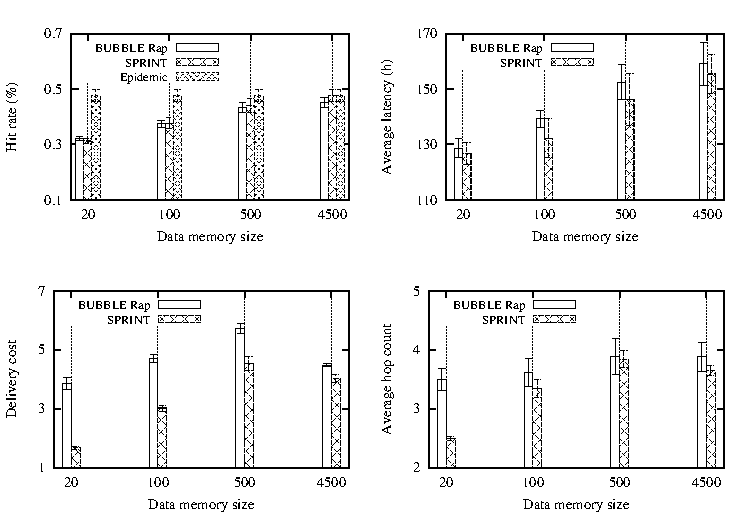
\includegraphics[scale=0.75]{img/upb2011}
		\caption{\label{fig:upb2011}UPB 2011 trace.}
	\end{figure}
\end{frame}

\begin{frame}{Results (St. Andrews)}
	\begin{figure}[!t]
		\centering
		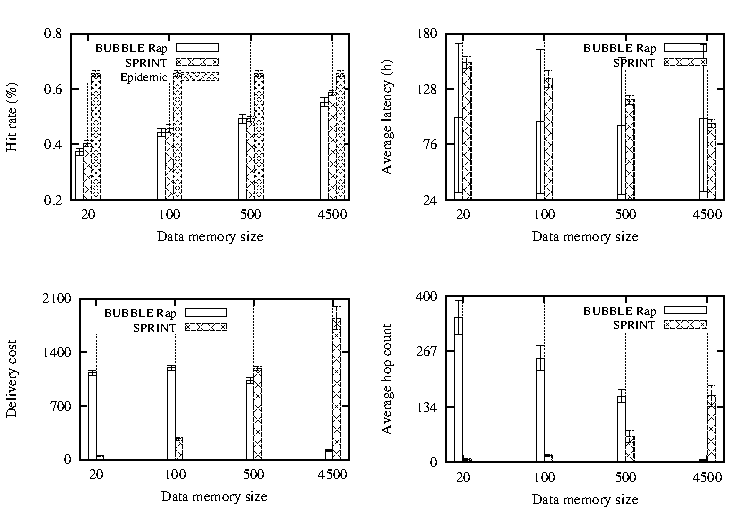
\includegraphics[scale=0.75]{img/stan}
		\caption{\label{fig:stan}St. Andrews trace.}
	\end{figure}
\end{frame}

\begin{frame}{Results (Content)}
	\begin{figure}[!t]
		\centering
		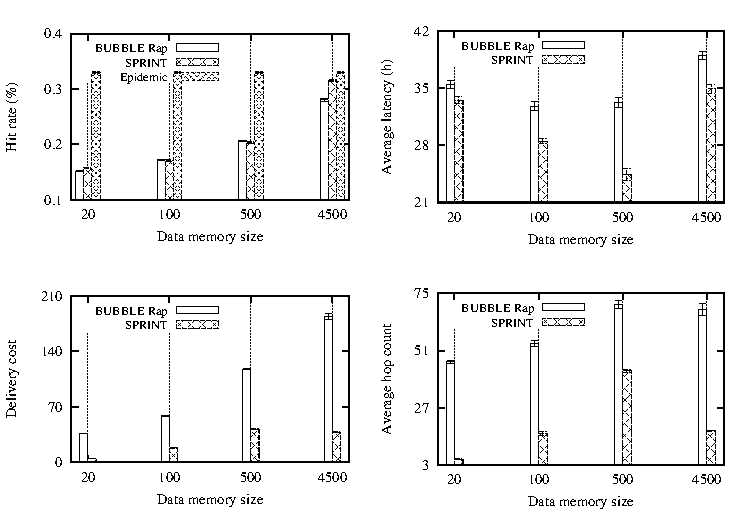
\includegraphics[scale=0.75]{img/content}
		\caption{\label{fig:content}Content trace.}
	\end{figure}
\end{frame}

\begin{frame}{Results (HCMM)}
	\begin{figure}[!t]
		\centering
		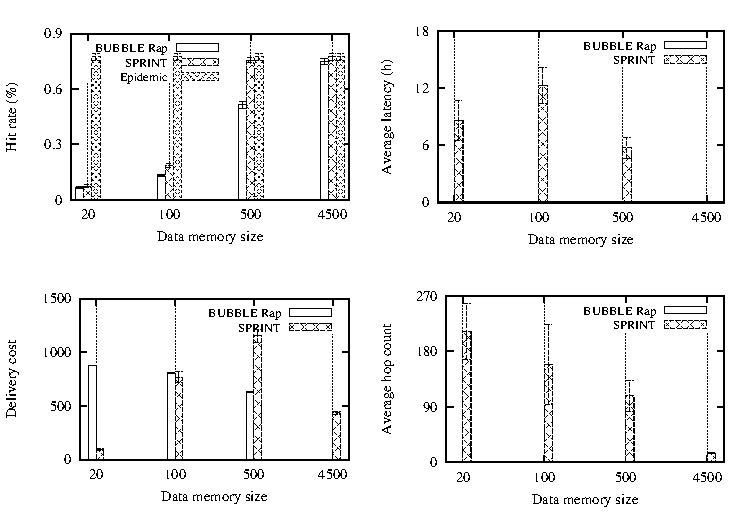
\includegraphics[scale=0.75]{img/hcmm}
		\caption{\label{fig:hcmm}HCMM model.}
	\end{figure}
	
	\tikz [remember picture,overlay]
    \node at
        ([yshift=7.5cm]current page.south) 
        %or: (current page.center)
        {
\includegraphics[scale=0.09]{img/deliver.png}};
\end{frame}

\begin{frame}{Selfish Nodes Detection [2]}
	\begin{itemize}
		\item selfish nodes $\rightarrow$ nodes that don’t want to participate in the routing process for various reasons
		\item propose a novel social-based collaborative content and context-based selfish node detection algorithm
		\item characteristics:
		\begin{itemize}
			\item an incentive mechanism that rewards active nodes and punishes selfish ones
			\item based on gossiping
			\item context-based: social knowledge, battery level, etc.
			\item content-based: message content-based decisions
		\end{itemize}
	\end{itemize}
	\vskip10pt
	\tiny{
	[2] Radu Ioan Ciobanu, Ciprian Dobre, Mihai Dascalu, Stefan Trausan-Matu and Valentin Cristea. 2013. Collaborative Selfish Node Detection with an Incentive Mechanism for Opportunistic Networks. In \emph{Proceedings of the 5th International Workshop on Management of the Future Internet} (ManFI '13).}
\end{frame}

\section{Conclusions}

\begin{frame}{Conclusions}
  \begin{columns}
    \begin{column}[l]{0.7\textwidth}
      \begin{itemize}
        \item SPRINT $\rightarrow$ routing algorithm for ONs that uses information about a node's social connections, contacts history, and predictions of future encounters
		\item it outperforms existing algorithms for various mobility traces and models
		\item improves hit rate, delivery latency, hop count and delivery cost
		\item distribution of contacts in certain scenarios is highly predictable and can be approximated as Poisson
      \end{itemize}
    \end{column}
    \begin{column}[c]{0.3\textwidth}
      \begin{figure}
        
\includegraphics[scale=0.2]{img/question-mark}
      \end{figure}
    \end{column}
  \end{columns}
\end{frame}

\end{document}
